\documentclass[10pt]{beamer}\usepackage[]{graphicx}\usepackage[]{color}
%% maxwidth is the original width if it is less than linewidth
%% otherwise use linewidth (to make sure the graphics do not exceed the margin)
\makeatletter
\def\maxwidth{ %
  \ifdim\Gin@nat@width>\linewidth
    \linewidth
  \else
    \Gin@nat@width
  \fi
}
\makeatother

\definecolor{fgcolor}{rgb}{0.345, 0.345, 0.345}
\newcommand{\hlnum}[1]{\textcolor[rgb]{0.686,0.059,0.569}{#1}}%
\newcommand{\hlstr}[1]{\textcolor[rgb]{0.192,0.494,0.8}{#1}}%
\newcommand{\hlcom}[1]{\textcolor[rgb]{0.678,0.584,0.686}{\textit{#1}}}%
\newcommand{\hlopt}[1]{\textcolor[rgb]{0,0,0}{#1}}%
\newcommand{\hlstd}[1]{\textcolor[rgb]{0.345,0.345,0.345}{#1}}%
\newcommand{\hlkwa}[1]{\textcolor[rgb]{0.161,0.373,0.58}{\textbf{#1}}}%
\newcommand{\hlkwb}[1]{\textcolor[rgb]{0.69,0.353,0.396}{#1}}%
\newcommand{\hlkwc}[1]{\textcolor[rgb]{0.333,0.667,0.333}{#1}}%
\newcommand{\hlkwd}[1]{\textcolor[rgb]{0.737,0.353,0.396}{\textbf{#1}}}%
\let\hlipl\hlkwb

\usepackage{framed}
\makeatletter
\newenvironment{kframe}{%
 \def\at@end@of@kframe{}%
 \ifinner\ifhmode%
  \def\at@end@of@kframe{\end{minipage}}%
  \begin{minipage}{\columnwidth}%
 \fi\fi%
 \def\FrameCommand##1{\hskip\@totalleftmargin \hskip-\fboxsep
 \colorbox{shadecolor}{##1}\hskip-\fboxsep
     % There is no \\@totalrightmargin, so:
     \hskip-\linewidth \hskip-\@totalleftmargin \hskip\columnwidth}%
 \MakeFramed {\advance\hsize-\width
   \@totalleftmargin\z@ \linewidth\hsize
   \@setminipage}}%
 {\par\unskip\endMakeFramed%
 \at@end@of@kframe}
\makeatother

\definecolor{shadecolor}{rgb}{.97, .97, .97}
\definecolor{messagecolor}{rgb}{0, 0, 0}
\definecolor{warningcolor}{rgb}{1, 0, 1}
\definecolor{errorcolor}{rgb}{1, 0, 0}
\newenvironment{knitrout}{}{} % an empty environment to be redefined in TeX

\usepackage{alltt}
\usetheme[10pt]{Singapore}
\usecolortheme{beaver}
\IfFileExists{upquote.sty}{\usepackage{upquote}}{}
\begin{document}

\title{The Trial}
\author{Chris Kozak}

\begin{frame}
  \titlepage
\end{frame}

\begin{frame}
  \frametitle{Outline}
    \tableofcontents
\end{frame}

\section{Load Packages}
\begin{frame}[fragile]
  \frametitle{Load Packages}
    \begin{itemize}
      \item
\begin{knitrout}
\definecolor{shadecolor}{rgb}{0.969, 0.969, 0.969}\color{fgcolor}\begin{kframe}
\begin{alltt}
\hlkwd{library}\hlstd{(dplyr)} \hlcom{#for querying data}
\end{alltt}
\end{kframe}
\end{knitrout}
      \item
\begin{knitrout}
\definecolor{shadecolor}{rgb}{0.969, 0.969, 0.969}\color{fgcolor}\begin{kframe}
\begin{alltt}
\hlkwd{library}\hlstd{(ggplot2)} \hlcom{#for visualizing data}
\end{alltt}
\end{kframe}
\end{knitrout}
      \item
\begin{knitrout}
\definecolor{shadecolor}{rgb}{0.969, 0.969, 0.969}\color{fgcolor}\begin{kframe}
\begin{alltt}
\hlkwd{library}\hlstd{(gutenbergr)} \hlcom{#for open-source docs}
\end{alltt}
\end{kframe}
\end{knitrout}
      \item
\begin{knitrout}
\definecolor{shadecolor}{rgb}{0.969, 0.969, 0.969}\color{fgcolor}\begin{kframe}
\begin{alltt}
\hlkwd{library}\hlstd{(stringr)} \hlcom{#for working with text data}
\end{alltt}
\end{kframe}
\end{knitrout}
      \item
\begin{knitrout}
\definecolor{shadecolor}{rgb}{0.969, 0.969, 0.969}\color{fgcolor}\begin{kframe}
\begin{alltt}
\hlkwd{library}\hlstd{(easyGgplot2)} \hlcom{#easily renders plots together}
\end{alltt}
\end{kframe}
\end{knitrout}
      \item
\begin{knitrout}
\definecolor{shadecolor}{rgb}{0.969, 0.969, 0.969}\color{fgcolor}\begin{kframe}
\begin{alltt}
\hlkwd{library}\hlstd{(tidytext)} \hlcom{#for quantifying sentiment in text}
\end{alltt}
\end{kframe}
\end{knitrout}
    
    \end{itemize}
\end{frame}

\section{The Trial}
\begin{frame}[fragile]
  \frametitle{About The Trial}
German author Franz Kafka wrote The Trial around 1915, but it wasn't published until 1925, after his death. It's the bleak, authoritarian story of a man on a trial for a crime he's not even aware of. This version was translated by David Wyllie. Naturally, other translations may feature different word choices, as the translator's goal here is to adapt a book written in an older style of German to a much newer style of English.
\end{frame}

\begin{frame}[fragile]
  \frametitle{Download The Trial}
\begin{knitrout}
\definecolor{shadecolor}{rgb}{0.969, 0.969, 0.969}\color{fgcolor}\begin{kframe}
\begin{alltt}
\hlstd{trial} \hlkwb{<-} \hlkwd{gutenberg_download}\hlstd{(}\hlnum{7849}\hlstd{)} \hlcom{#download The Trial}
\hlkwd{head}\hlstd{(trial}\hlopt{$}\hlstd{text)} \hlcom{#preview the text}
\end{alltt}
\begin{verbatim}
## [1] "The Trial"                                  
## [2] "Franz Kafka"                                
## [3] ""                                           
## [4] "Translation Copyright (C) by David Wyllie"  
## [5] "Translator contact email: dandelion@post.cz"
## [6] ""
\end{verbatim}
\end{kframe}
\end{knitrout}
\end{frame}

\section{Unnest the Tokens}
\begin{frame}[fragile]
  \frametitle{Unnest the Tokens}
\begin{knitrout}
\definecolor{shadecolor}{rgb}{0.969, 0.969, 0.969}\color{fgcolor}\begin{kframe}
\begin{alltt}
\hlstd{trial_words} \hlkwb{<-} \hlstd{trial}\hlopt
  \hlkwd{unnest_tokens}\hlstd{(word, text)} \hlcom{#separates each word}
\hlstd{trial_words}\hlopt{$}\hlstd{gutenberg_id} \hlkwb{<-} \hlkwa{NULL}
\end{alltt}
\end{kframe}
\end{knitrout}
\end{frame}

\section{Bing Sentiment Lexicon}
\begin{frame}[fragile]
  \frametitle{Bing Sentiment Lexicon}
\begin{knitrout}
\definecolor{shadecolor}{rgb}{0.969, 0.969, 0.969}\color{fgcolor}\begin{kframe}
\begin{alltt}
  \hlcom{#for positive/negative sentiments}
  \hlstd{bing} \hlkwb{<-} \hlkwd{get_sentiments}\hlstd{(}\hlstr{'bing'}\hlstd{)}

  \hlkwd{head}\hlstd{(bing)} \hlcom{#preview bing}
\end{alltt}
\begin{verbatim}
## # A tibble: 6 x 2
##         word sentiment
##        <chr>     <chr>
## 1    2-faced  negative
## 2    2-faces  negative
## 3         a+  positive
## 4   abnormal  negative
## 5    abolish  negative
## 6 abominable  negative
\end{verbatim}
\end{kframe}
\end{knitrout}
\end{frame}

\begin{frame}[fragile]
  \frametitle{Merging the Lexicon}
\begin{knitrout}
\definecolor{shadecolor}{rgb}{0.969, 0.969, 0.969}\color{fgcolor}\begin{kframe}
\begin{alltt}
  \hlcom{#merge bing with The Trial}
  \hlstd{trial_words} \hlkwb{<-} \hlkwd{inner_join}\hlstd{(trial_words,bing)}
  \hlstd{trial_words}\hlopt{$}\hlstd{gutenberg_id}\hlkwb{<-}\hlkwa{NULL} \hlcom{#delete extra column}
  \hlkwd{head}\hlstd{(trial_words)} \hlcom{#preview the dataframe/tibble}
\end{alltt}
\begin{verbatim}
## # A tibble: 6 x 2
##           word sentiment
##          <chr>     <chr>
## 1         miss  negative
## 2         lies  negative
## 3        wrong  negative
## 4      unusual  negative
## 5 disconcerted  negative
## 6        knock  negative
\end{verbatim}
\end{kframe}
\end{knitrout}
\end{frame}

\section{Data Transformation}
\begin{frame}[fragile]
  \frametitle{Positive Words Transformation}
\begin{knitrout}
\definecolor{shadecolor}{rgb}{0.969, 0.969, 0.969}\color{fgcolor}\begin{kframe}
\begin{alltt}
\hlstd{trial_pos} \hlkwb{<-} \hlstd{trial_words}\hlopt
  \hlkwd{filter}\hlstd{(sentiment}\hlopt{==}\hlstr{'positive'}\hlstd{)}\hlopt
  \hlkwd{group_by}\hlstd{(word)}\hlopt
  \hlkwd{summarize}\hlstd{(}\hlkwc{count}\hlstd{=}\hlkwd{n}\hlstd{(),} \hlkwc{sentiment}\hlstd{=}\hlkwd{first}\hlstd{(sentiment))}\hlopt
  \hlkwd{arrange}\hlstd{(count)}\hlopt
  \hlkwd{top_n}\hlstd{(}\hlnum{15}\hlstd{,} \hlkwc{wt}\hlstd{=count)}

\hlstd{trial_pos}\hlopt{$}\hlstd{word} \hlkwb{<-} \hlkwd{factor}\hlstd{(trial_pos}\hlopt{$}\hlstd{word,}
                         \hlkwc{levels}\hlstd{=trial_pos}\hlopt{$}\hlstd{word)}

\hlstd{pos_plot} \hlkwb{<-} \hlkwd{ggplot}\hlstd{()}\hlopt{+}
  \hlkwd{geom_bar}\hlstd{(}\hlkwc{data} \hlstd{= trial_pos,}
           \hlkwd{aes}\hlstd{(}\hlkwc{x}\hlstd{=word,} \hlkwc{y}\hlstd{=count),} \hlkwc{stat}\hlstd{=}\hlstr{'identity'}\hlstd{,} \hlkwc{fill}\hlstd{=}\hlstr{'blue'}\hlstd{)}\hlopt{+}
  \hlkwd{coord_flip}\hlstd{()}\hlopt{+}
  \hlkwd{ggtitle}\hlstd{(}\hlstr{'Positive words'}\hlstd{)}
\end{alltt}
\end{kframe}
\end{knitrout}
\end{frame}

\section{Positive Words}
\begin{frame}[fragile]
  \frametitle{Positive Plot}
\begin{knitrout}
\definecolor{shadecolor}{rgb}{0.969, 0.969, 0.969}\color{fgcolor}\begin{kframe}
\begin{alltt}
\hlstd{pos_plot}
\end{alltt}
\end{kframe}
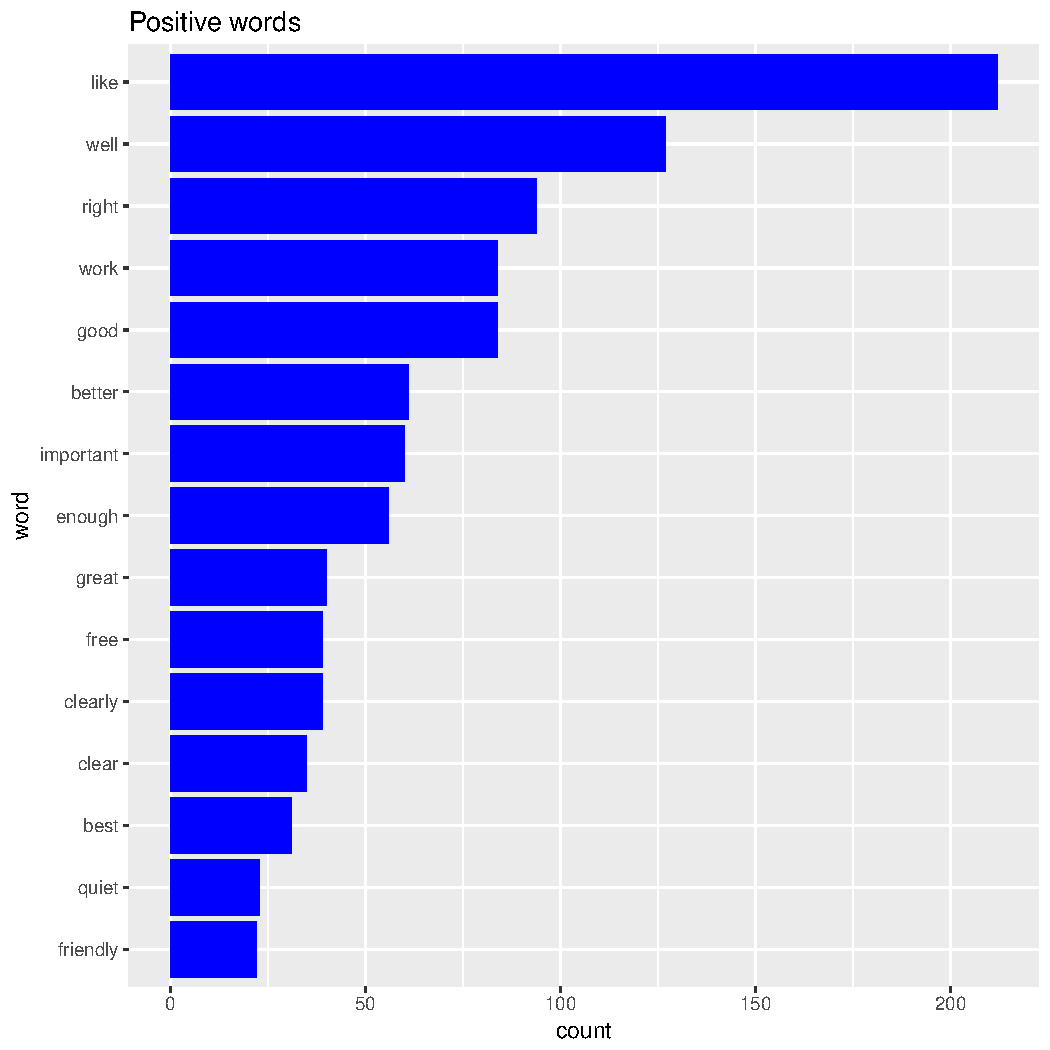
\includegraphics[width=\maxwidth]{figure/unnamed-chunk-12-1} 

\end{knitrout}
\end{frame}

\section{Negative Words}
\begin{frame}[fragile]
  \frametitle{Negative Words Transformation}
\begin{knitrout}
\definecolor{shadecolor}{rgb}{0.969, 0.969, 0.969}\color{fgcolor}\begin{kframe}
\begin{alltt}
\hlstd{trial_neg} \hlkwb{<-} \hlstd{trial_words}\hlopt
  \hlkwd{filter}\hlstd{(sentiment}\hlopt{==}\hlstr{'negative'}\hlstd{)}\hlopt
  \hlkwd{group_by}\hlstd{(word)}\hlopt
  \hlkwd{summarize}\hlstd{(}\hlkwc{count}\hlstd{=}\hlkwd{n}\hlstd{(),}
            \hlkwc{sentiment}\hlstd{=}\hlkwd{first}\hlstd{(sentiment))}\hlopt
  \hlkwd{arrange}\hlstd{(count)}\hlopt
  \hlkwd{top_n}\hlstd{(}\hlnum{15}\hlstd{,} \hlkwc{wt}\hlstd{=count)}

\hlstd{trial_neg}\hlopt{$}\hlstd{word} \hlkwb{<-} \hlkwd{factor}\hlstd{(trial_neg}\hlopt{$}\hlstd{word,}
                         \hlkwc{levels}\hlstd{=trial_neg}\hlopt{$}\hlstd{word)}

\hlstd{neg_plot} \hlkwb{<-} \hlkwd{ggplot}\hlstd{()}\hlopt{+}
  \hlkwd{geom_bar}\hlstd{(}\hlkwc{data} \hlstd{= trial_neg,}
           \hlkwd{aes}\hlstd{(}\hlkwc{x}\hlstd{=word,} \hlkwc{y}\hlstd{=count),} \hlkwc{stat}\hlstd{=}\hlstr{'identity'}\hlstd{,} \hlkwc{fill}\hlstd{=}\hlstr{'red'}\hlstd{)}\hlopt{+}
  \hlkwd{coord_flip}\hlstd{()}\hlopt{+}
  \hlkwd{ggtitle}\hlstd{(}\hlstr{'Negative words'}\hlstd{)}
\end{alltt}
\end{kframe}
\end{knitrout}
\end{frame}

\begin{frame}[fragile]
  \frametitle{Negative Plot}
\begin{knitrout}
\definecolor{shadecolor}{rgb}{0.969, 0.969, 0.969}\color{fgcolor}\begin{kframe}
\begin{alltt}
\hlstd{neg_plot}
\end{alltt}
\end{kframe}
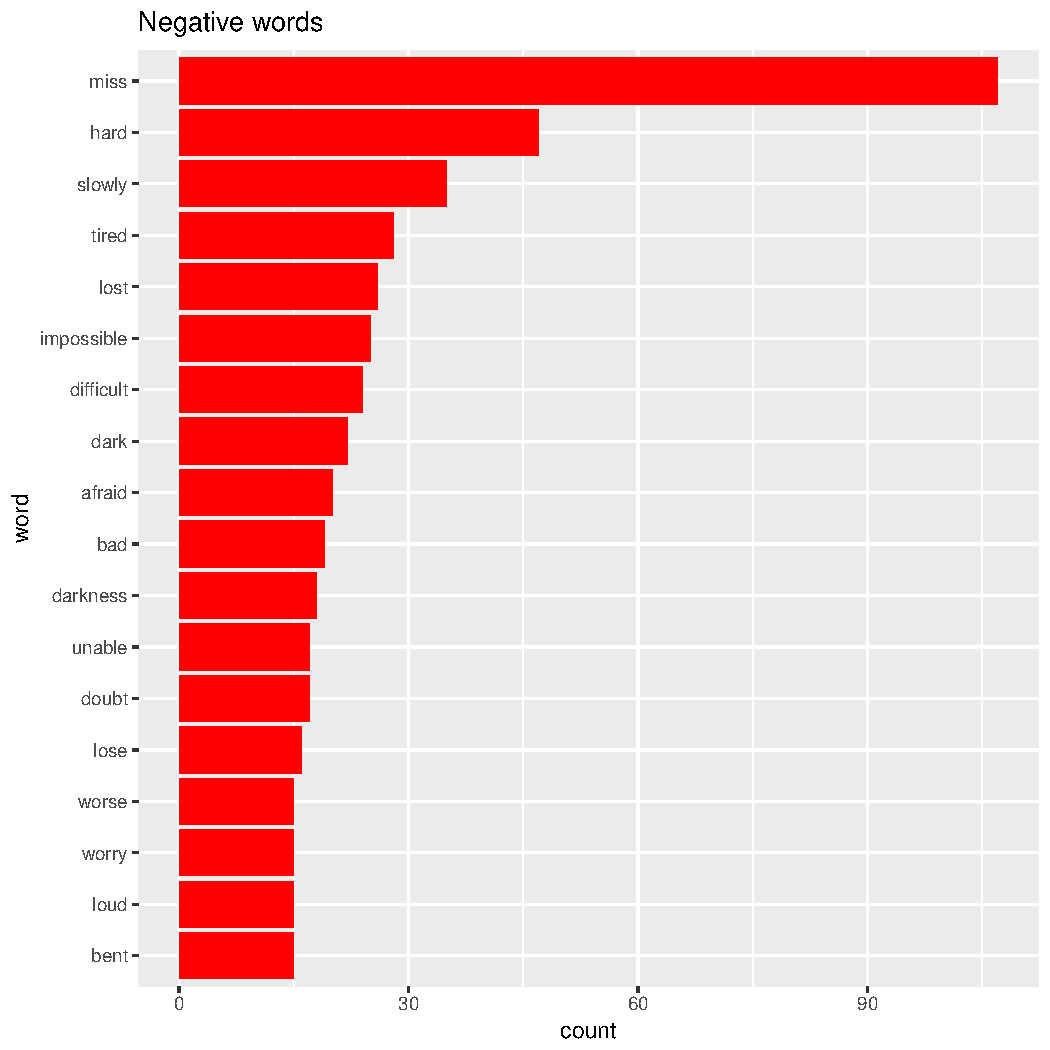
\includegraphics[width=\maxwidth]{figure/unnamed-chunk-14-1} 

\end{knitrout}

\end{frame}
\end{document}
